Observa la recta numérica. El punto A está en \(-3\) y el punto B en \(2\). Si desde A nos movemos 5 unidades hacia la derecha y luego 3 hacia la izquierda, ¿en qué número terminamos? Representa el movimiento en la recta.

\begin{center}
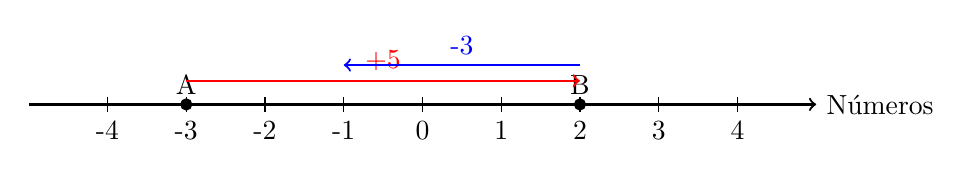
\begin{tikzpicture}
    \draw[thick, ->] (-5,0) -- (5,0) node[right] {Números};
    \foreach \x in {-4,-3,-2,-1,0,1,2,3,4}
        \draw (\x,0.1) -- (\x,-0.1) node[below] {\x};
    % Puntos A y B
    \filldraw (-3,0) circle (2pt) node[above] {A};
    \filldraw (2,0) circle (2pt) node[above] {B};
    % Flechas de movimiento
    \draw[->, red, thick] (-3,0.3) -- (2,0.3) node[midway, above] {+5};
    \draw[->, blue, thick] (2,0.5) -- (-1,0.5) node[midway, above] {-3};
\end{tikzpicture}
\end{center}